\documentclass[12pt,a4paper]{article}

\input{../../preamble_files/packages}
\input{../../preamble_files/scriptr}
\input{../../preamble_files/siunits}
\input{../../preamble_files/vectors}
\input{../../preamble_files/figures}
\input{../../preamble_files/references}
\input{../../preamble_files/empheq}

\pagestyle{fancy}
\lhead{Richard Whitehill}
\chead{PHYS 631 -- HW E}
\rhead{02/03/22}
\cfoot{\thepage \hspace{1pt} of \pageref{LastPage}}

\newcommand{\prob}[2]{\textbf{#1)} #2}

\setlength{\parskip}{\baselineskip}
\setlength{\parindent}{0pt}

\begin{document}

\prob{2.13}{Find the electric field a distance $s$ from an infinitely long straight wire that carries a uniform line charge $\lambda$. Compare Eq. 2.9.}

For this problem, the setup is rotationally symmetric about the wire, so we will use Gauss's Law with a cylindrical Gaussian surface of radius $s$.

\bef
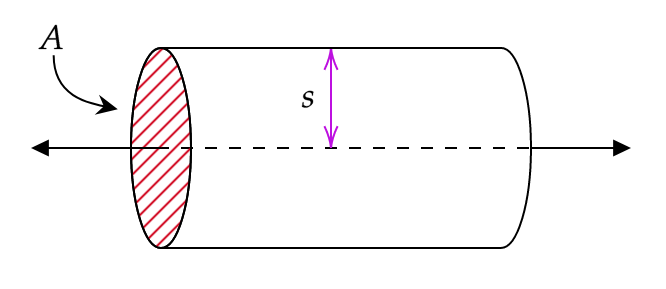
\includegraphics[scale=0.5]{fig1.png}
\eef

Gauss's law tells us that
\begin{align*}
\oint \va*{E} \vdot \dd{\va*{a}} = \frac{Q_{\rm enc}}{\epsilon_0} = \frac{\lambda \ell}{\epsilon_0}
\end{align*}

It is observed that contribution to the flux through the ends of the cylinder is zero, so only obtain a radial component, pointing normal to the curved surface of the cylinder.
\begin{align*}
E\qty(2\pi s \ell) = \frac{\lambda \ell}{\epsilon_0}
\end{align*}

\begin{eqbox}
\va*{E} = \frac{1}{2\pi\epsilon_0}\frac{\lambda}{s} \shat = \frac{1}{4\pi\epsilon_0}\frac{2\lambda}{s} \shat
\end{eqbox}

Notice that this is the same as Eq. 2.9, since the $z$ axis in that example is not uniquely defined since we could rotate about the wire and end up with an equivalent physical setup.

\prob{2.17}{An infinite plane slab, of thickness $2d$, carries a uniform volume charge density $\rho$. Find the electric field, as a function of $y$, where $y = 0$ at the center. Plot $E$ versus $y$, calling $E$ positive when it points in the $+y$ direction and negative when it points in the $-
y$ direction.}

In the figure below, we see the slab set up. Note that it extends infinitely in the $x$ and $z$ directions. For this problem, we can set up a Gaussian surface, which is a cylinder with a height $2y$. Note that there are two cases: $|y| < d$ or $|y| \geq d$ shown in the left and right figures.

\bef
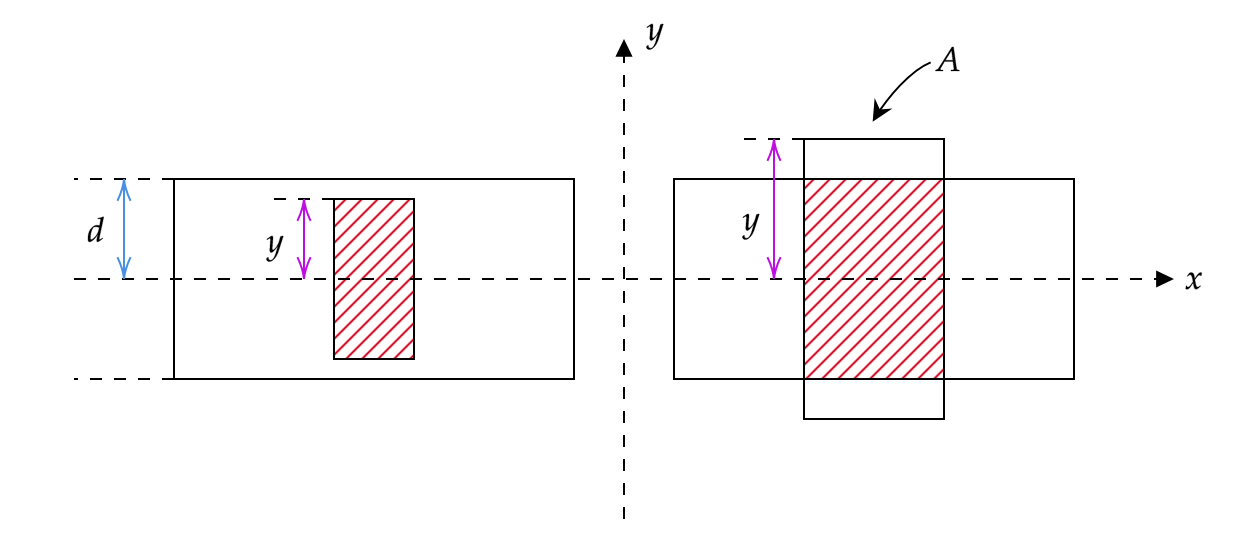
\includegraphics[scale=0.35]{fig2.png}
\eef

Since there is rotational symmetry in the $xz$-plane, the only component of the electric field is in the $y$ direction. From Gauss's law, we have
\begin{align*}
\oint \va*{E} \vdot \dd{\va*{a}} &= 2A|E| = \frac{Q_{\rm enc}}{\epsilon_0} = \frac{A}{\epsilon_0}\int \rho(y) \dd{y} \\
\Rightarrow |E| &= \frac{1}{2\epsilon}\int \rho(y) \dd{y}
\end{align*}

Note that $\rho$ is constant inside the slab and $\rho = 0$ outside the slab, so the integral over $y$ gives
\begin{eqbox}
|E| = \frac{\rho}{\epsilon_0}\begin{cases}
y, & |y| < d \\
d, & |y| \geq d
\end{cases}
\end{eqbox}

Notice that the electric field linearly increases as a function of $y$ and is constant outside of the slab, pointing away from the $xz$ plane. A plot of this is shown below.

\bef
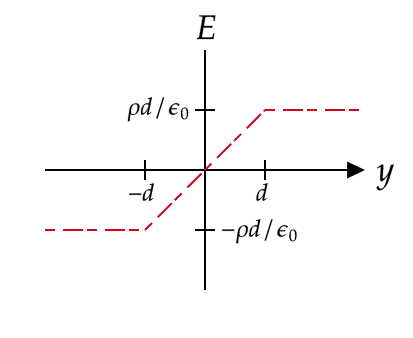
\includegraphics[scale=0.6]{fig3.png}
\eef

\end{document}
